\documentclass[12pt,openany]{book}

%PACKAGES%
\usepackage[inner=25.86mm, outer=18.24mm, top=25.86mm, bottom=33.48mm, papersize={154mm, 216mm}]{geometry}
\usepackage{graphicx}
\usepackage[polish]{babel}
\usepackage{fontspec}
\usepackage{enumitem}
\usepackage{sectsty}
\usepackage[]{titlesec}
\usepackage{verse}
\usepackage{fix-cm}%font size
\usepackage{multirow}%tables
\usepackage{array}%tables
\usepackage[hyphens]{url}
% \usepackage{tocloft}
\usepackage{soulutf8}
\usepackage{marginnote}

\renewcommand*{\marginfont}{\SkolarLight}

%this snippet of code is a bit of a hack to allow line break after em-dash (http://tex.stackexchange.com/questions/62800/lualatex-and-line-breaks-after-em-dashes)
\catcode`\—=13
\protected\def—{\unskip\textemdash\allowbreak}

%\usepackage{pagegrid}
%PACKAGES%
%\pagegridsetup{top-left, step=3.435in}


%LINESPACE% SETS LINESPA\caps{ce}
\usepackage{setspace}
\setstretch{1.15}
%LINESPACE%

%FONTS% 
\setmainfont[Numbers=OldStyle]{Alegreya}
\setsansfont[Scale = MatchLowercase]{Alegreya Sans}
\setmonofont{Alegreya}

\newfontfamily\Chapfont[ItalicFont=Alegreya Sans Italic]{Alegreya Sans}
\chapterfont{\Chapfont\LARGE\centering\mdseries\setstretch{1}}
\newfontfamily\Secfont[Numbers=OldStyle]{Alegreya Sans Medium}
\sectionfont{\Secfont\mdseries\large\setstretch{1}}

%HEADINGS%

%HEADER% 
\usepackage{fancyhdr, textcase}
\setlength{\headheight}{15pt}
\pagestyle{fancy}
\renewcommand{\chaptermark}[1]{\markboth{\thechapter.\ #1}{}}
\renewcommand{\sectionmark}[1]{\markright{\thesection\ #1}}

\fancyhf{}
\fancyhead[LE,RO]{\thepage}
\fancyhead[CO]{\headcaps{\MakeUppercase{Ajahn Brahmali}}}
\renewcommand{\headrulewidth}{0pt}
\fancypagestyle{plain}{ %
\fancyhf{} % remove everything
\renewcommand{\headrulewidth}{0pt}
\renewcommand{\footrulewidth}{0pt}}
\newfontfamily\headcapsfont[RawFeature=+c2sc]{Alegreya}
\newcommand\headcaps[1]{{\headcapsfont #1}}
\fancyhead[CE]{\headcaps{\MakeUppercase{Samatha \& Vipassanā}}}
%HEADER%

%HANGING LEFT%
\newcommand*{\vleftofline}[1]{\leavevmode\llap{#1}}
%HANGINGLEFT%

%WIDOWS & ORPHANS% 
\widowpenalty=10000
\clubpenalty=10000
%WIDOWS & ORPHANS%

%Applies various subtle improvements in typography. Use default.
\usepackage{microtype}
\frenchspacing

\usepackage[unicode, hidelinks, pdfauthor={Brahmali}, pdftitle={Dlaczego Samatha i Vipassanā są nierozerwalne}, pdfsubject={Buddyzm}, pdfkeywords={Buddyzm, bhikkhu, mnisi, sutta, tipitaka, tripitaka, sutra, samatha, vipassana, spokój, wgląd}, pdfproducer={LuaTeX  beta-0.70.1}, pdfcreator={LaTeX2e}]{hyperref}

%DOCUMENT INFO. NOT USED IN TEXT.%
\title{ Dlaczego \protect\\ Samatha i Vipassanā \protect\\ są nierozerwalne}
\author{Ajahn Brahmali}
\date{}
\begin{document}
\frontmatter
\pagestyle{empty}
\newgeometry{margin=0pt}

\hspace*{-156mm}
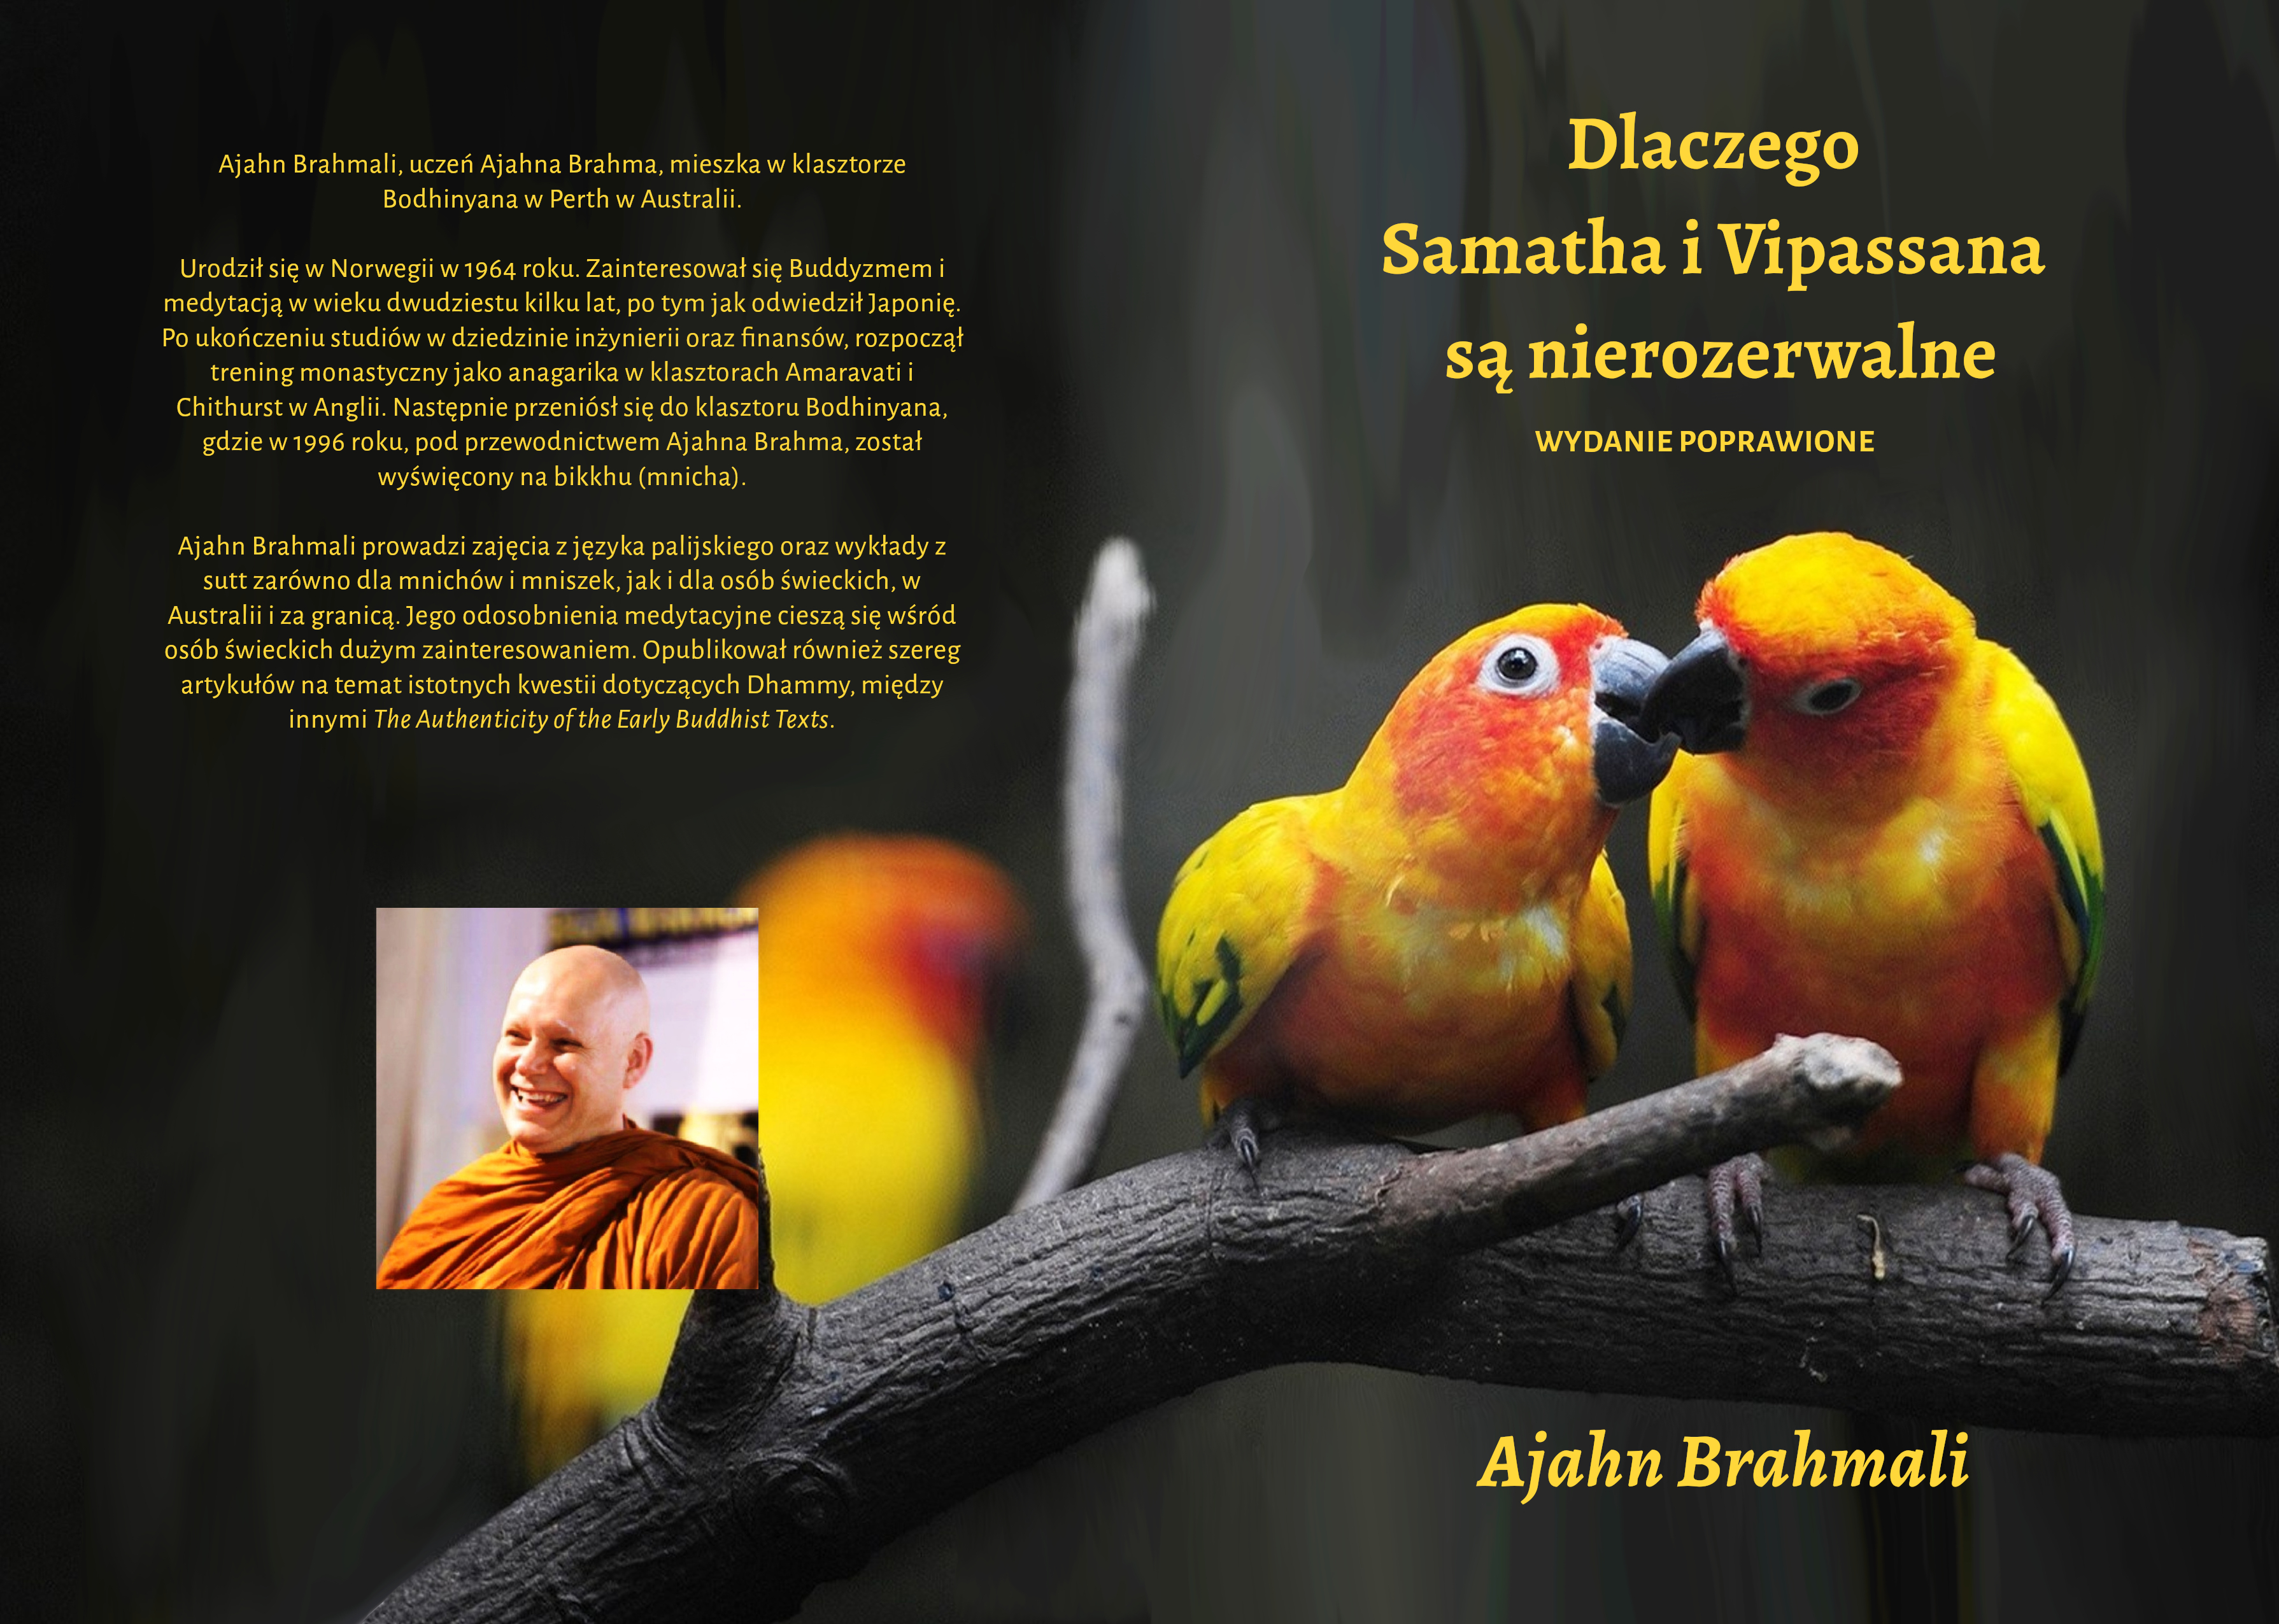
\includegraphics{sv-2_a5_cover.png}

% \begin{center}

% \vfill

% \maketitle

% \vfill
% \end{center}

\restoregeometry

\begin{center}\end{center}

\vspace{4em}
{\small
\noindent W oparciu o mowę wygłoszoną w piątek, 8 maja, 2015 \\w Dhammaloka Buddhist Centre, Perth, Australia.

\bigskip

\noindent Prawa autorskie Ajahn Brahmali.

\medskip

\noindent Tytuł oryginału:  Why Samatha and Vipassanā are Inseparable

\bigskip

\noindent Opracowanie i wydanie:

\medskip

\noindent Ajahn Brahm Society of Sri Lanka

\noindent 380/9, Sarana Road, Colombo 7, Sri Lanka

\noindent abs.sl.list@gmail.com

\bigskip

\noindent Polskie tłumaczenie 2023:

\medskip

\noindent Tłumaczenie: Karolina Laube

\noindent Korekta: Natalia Gołębiewska

\noindent Skład: Remy Jakobson, Ven. Vimala

}

\vfill

\begin{center}
\textit{ Niech wszystkie istoty będą szczęśliwe!}

\end{center}
\vfill

\newpage

\begin{center}\end{center}
\begin{center}

\vfill

{\huge \textit{Dlaczego} 

\medskip

\textbf{Samatha} \textit{i} \textbf{Vipassanā} 

\bigskip

\textit{są nierozerwalne}}

\vfill

\caps{\LARGE Ajahn Brahmali}

\vfill
\end{center}

 \newpage

\begin{center}\end{center}
\begin{center}

\vfill

\textit{\large Brak mi słów, kiedy ludzie pytają mnie: \\„Czy nauczasz medytacji vipassanā?”}

\vfill

\end{center}

\newpage
\mainmatter
\chapter*{Wstęp}

Dość często ludzie dzwonią do naszego klasztoru w Perth, pytając czy nauczamy medytacji \textit{vipassanā}. Brak mi słów, kiedy ludzie zadają to pytanie, i odpowiadam: „Tak, z jednej strony można powiedzieć, że tak, uczymy medytacji \textit{vipassanā}, ale z drugiej strony chyba jednak nie”. Albo mówię: „Nauczamy buddyjskiej medytacji”, albo coś w tym rodzaju. Nie chcę, żeby ktoś dla kogo Dhamma i praktyka medytacji są nowe, wziął to za zbyt skomplikowane bądź kontrowersyjne.

\textit{Samatha} i \textit{vipassanā} są kluczowe w buddyjskiej praktyce medytacji. \textit{Samatha} jest zazwyczaj tłumaczona jako spokój, wyciszenie, podczas gdy \textit{vipassanā} jest tłumaczona jako wgląd. Poniżej zamierzam omówić, na ile odpowiednie są te tłumaczenia. W tym celu, musimy zrozumieć, jak Buddha używał tych słów.

\chapter*{Problem z medytacją „\textit{vipassanā}”}

\pagestyle{fancy}

W \textit{suttach}, Buddha mówi o \textit{vipassanā} i o medytacji, ale nigdy nie łączy tych dwóch słów w „medytację \textit{vipassanā}”. Pomimo powszechnego użycia tego terminu współcześnie, faktem jest, że Buddha nigdy go nie używał. Czym zatem jest \textit{vipassanā}? I jaki ma związek z \textit{samatha}? To są główne zagadnienia, które omawiam w tym eseju.

Łatwo zrozumieć zainteresowanie ludzi medytacją \textit{vipassanā}. To brzmi atrakcyjnie i skutecznie. Kto nie chciałby mieć wglądu? Wgląd oznacza mądrość, zrozumienie, jasność spraw. Oznacza poznanie swojego ciała i umysłu, zrozumienie własnego wszechświata i wgląd w jego naturę. Mądrość jest najważniejszą zdolnością umysłową dla osobistego poczucia sensu i szczęścia. Kiedy słyszę „medytacja wglądu”, myślę sobie: „Wow, medytacja, która prowadzi do mądrości; to jest właśnie to, czego chcę”. Medytacja wglądu to potężne wyrażenie i prawdopodobnie właśnie dlatego stało się ono tak popularne. Mimo to, Buddha nigdy go nie używał.

Istnieją dobre powody, dla których Buddha nigdy nie wspominał o medytacji \textit{vipassanā}. Jedną z konsekwencji używania tego zwrotu jest oddzielenie \textit{samatha} od \textit{vipassanā}. Mówiąc o medytacji wglądu, sugerujesz, że istnieje coś innego, co nazywa się medytacją spokoju. Ale Buddha nigdy nie używał zwrotu „medytacja spokoju”. W \textit{suttach}, \textit{samatha} i \textit{vipassanā}, spokój i wgląd, są rezultatem praktyki, a nie praktykami samymi w sobie. I zwykle są one połączone, stanowiąc dwa aspekty tego samego procesu rozwoju umysłowego.

Co więcej, kiedy skupiasz się na medytacji wglądu i nadajesz jej ważność, sugerujesz, że pozostałe medytacje, szczególnie medytacja spokoju są mniej ważne. Sam fakt, że kładziesz nacisk na jedną, sugeruje coś na temat drugiej, nawet jeśli nie jest to powiedziane wprost. To kolejny powód, dla którego uważam, że mówienie o medytacji wglądu jest niefortunne: prowadzi ono do wydawania osądu na temat tego, co tak naprawdę jest ważne na ścieżce buddyjskiej.

\chapter*{\textit{Samatha} i \textit{vipassanā}: co naprawdę oznaczają}

Zanim omówimy proces medytacji w szczegółach, przyjrzyjmy się znaczeniu  \textit{samatha} i \textit{vipassanā}.

\section*{\textit{Samatha}}

Znaczenie słowa \textit{samatha} nie jest niczym kontrowersyjnym. Używane jest zarówno w \textit{suttach}, jak i w \textit{vinayi}, i w niedwuznaczny sposób odnosi się do spokoju i wyciszenia, zarówno zewnętrznego, w społeczności, jak i wewnętrznego, w naszym osobistym doświadczeniu. Każdy, kto kiedykolwiek medytował, będzie miał pojęcie, czym to osobiste doświadczenie jest. Kiedy siadasz i zamykasz oczy, a twoja medytacja idzie dobrze, po pewnym czasie czujesz się spokojniejszy. Co to oznacza? To oznacza, że twój umysł jest mniej rozbiegany. To oznacza, że w twoim umyśle jest mniej pragnień i splamień. To oznacza, że czujesz się bardziej zrelaksowany i spokojny. To jest bardzo pozytywne doświadczenie. Uczucie spokoju jest lepsze niż uczucie poruszenia, niepokoju i pożądania.

Ciekawą sprawą jest to, że spokój, który odczuwasz po dobrej medytacji to tylko początek pięknej buddyjskiej drogi. Krok po kroku, poczucie spokoju wzrasta i przekształca się w niewyobrażalne wcześniej poczucie spokoju i wyciszenia. W tym spokoju jest głębia. Kiedy tego doświadczasz, zaczynasz rozumieć, dlaczego medytacja jest tak wyjątkowa, do tego stopnia, że pozwala ci dotknąć sensu życia. Stopniowo wszystko staje się niesamowicie spokojne i nieruchome. Twój dotychczasowy świat znika i widzisz wszystko w zupełnie nowym świetle.

A więc spokój to rzecz względna. Myślisz, że stałeś się spokojniejszy po medytacji, ale z czasem stajesz się jeszcze bardziej spokojny. Spoglądając wstecz na poprzednią medytację, myślisz sobie: „Hej, to w ogóle nie był spokój; to był niepokój!”. Potem stajesz się jeszcze bardziej spokojny, ale znowu spoglądając wstecz, myślisz sobie: „To też nie był spokój”. Kontynuując w ten sposób, krok po kroku, zaczynasz nabierać właściwej perspektywy na życie. Im jesteś spokojniejszy, tym lepiej rozumiesz cierpienie i sens życia. Bycie naprawdę spokojnym jest zarówno transformujące, jak i błogie. W końcu przenosisz to na bardzo głęboki poziom.

To jest \textit{samatha}.

\section*{\textit{Vipassanā}}

Po drugiej stronie naszej pary \textit{samatha}\textit{-vipassanā} jest \textit{vipassanā}, \linebreak często tłumaczona jako wgląd. Zacznijmy od tego, że musimy \linebreak zdecydować, na ile trafny jest taki przekład. Po dość szczegółowym przestudiowaniu nauk Buddhy, myślę, że to tłumaczenie można poprawić.

Z perspektywy lingwistycznej, \textit{vipassanā} składa się z przedrostka \textit{vi-} oraz słowa \textit{passanā}, które oznacza „widzenie”. Mamy więc do czynienia z konkretnym rodzajem widzenia, którego dokładny rodzaj jest określony przez przedrostek \textit{vi-}. Przedrostek \textit{vi-} jest używany w wielu różnych znaczeniach, z których dwa są najbardziej istotne z naszego punktu widzenia. Jednym z nich jest idea separacji. W tym sensie \textit{vi-} oznacza rozróżnienie albo analizę, a \textit{vipassanā} może być tłumaczona jako analityczne widzenie lub wgląd. Ale \textit{vi-} jest również używane do oznaczenia intensyfikacji, co może skłaniać do tłumaczenia \textit{vipassanā} jako „prawdziwego widzenia” albo „jasnego widzenia”. A zatem które tłumaczenie jest poprawne?

Jedna z \textit{sutt} w szczególności rzuca na to światło. W tej \textit{sutcie}, AN 2.31, powiedziane jest, że \textit{vipassanā} prowadzi do \textit{paññā}, mądrości. Jeśli przetłumaczymy \textit{vipassanā} jako wgląd, to znaczenie tej \textit{sutty} będzie takie, iż wgląd prowadzi do mądrości. Jednak w języku angielskim te dwa słowa, wgląd i mądrość, są prawie jednoznaczne, szczególnie w kontekście duchowości. Jeśli \textit{vipassanā} prowadzi do mądrości, to potrzebujemy takiej interpretacji \textit{vipassanā}, która nie oznacza mądrości samej w sobie, ale krok w jej stronę. Biorąc pod uwagę dwie dostępne opcje w naszej analizie lingwistycznej powyżej, jasne widzenie jest zatem lepszym tłumaczeniem niż wgląd.

Ale to nie wszystko. Według Mahāpadāna Sutta (DN 14), istniał poprzedni Buddha zwany Vipassī, co oznacza „tego, który ma \textit{vipassanā}”. Ta sama \textit{sutta} mówi, iż otrzymał takie imię ponieważ jego przeszła  \textit{kamma} uczyniła go jasnowidzącym od urodzenia i ponieważ był „bez mrugnięcia okiem czujny, jak bogowie Trzydziestu Trzech”. Oba te powody przemawiają za tłumaczeniem  \textit{vipassanā} jako jasnego widzenia, a nie wglądu.

W języku angielskim istnieje istotna różnica pomiędzy wglądem a jasnym widzeniem. Wgląd odnosi się do czegoś, co dzieje się nagle; „Wow, teraz rozumiem!”. Jest to chwila uświadomienia sobie, przebłysk w umyśle. Ta metafora jest używana również w \textit{suttach} do zobrazowania wejścia w strumień, głębokiego momen\-tu wglądu. Z kolei jasne widzenie to coś, co w różnym stopniu zawsze obecne jest w umyśle. W tej chwili, albo widzisz rzeczy jasno albo nie, albo jesteś gdzieś pomiędzy. Jeśli wyobrazisz sobie jasne widzenie jako skalę przesuwną, która zaczyna się od kompletnego zamętu, a kończy na pełnej jasności umysłu, to zawsze znajdujesz się w jakimś punkcie tej skali.

A więc w kontekście medytacji, twoja \textit{vipassanā} stopniowo \linebreak wzrasta wraz z postępem w medytacji. Po dobrej medytacji stajesz \textit{spokojniejszy} i masz więcej \textit{vipassanā}. Kiedy spoglądasz w siebie, z większą łatwością widzisz stan swojego umysłu. Zamiast pędzić od pomysłu do pomysłu, od jednego stanu mentalnego do drugiego, masz teraz wystarczającą jasność, aby zobaczyć, co w nim jest. Widzisz, że rzeczy powstają i zanikają. Widzisz splamienia --- ich powstawanie, obecność i zanikanie. Z perspektywy medytacji tym właśnie jest \textit{vipassanā}: zdolnością jasnego widzenia tego, co się dzieje, a zwłaszcza tego, co dzieje się w tobie.

Ten rodzaj jasnego widzenia jest krytyczną częścią ścieżki duchowej. Im większą masz świadomość tego, co się dzieje w twoim umyśle, tym większa szansa, że coś z tym zrobisz. Jasne widzenie to niezbędna podstawa, która pozwala ci zmienić perspektywę i sposób myślenia. Pozwala ci skierować życie w nowym kierunku, w stronę zdrowych cech, w stronę tego, co prowadzi do szczęścia, a nie do cierpienia. W miarę postępów na ścieżce, jasne widzenie staje się coraz bardziej subtelne. Im większy spokój w medytacji, tym jaśniej widzisz i masz większą zdolność kierowania umysłu w dobrą stronę.

Nie tylko widzisz splamienia, ale widzisz również ich przyczyny. Idea przyczynowości jest bardzo istotna w buddyzmie. \linebreak Dlaczego myślisz w określony sposób? Dlaczego postrzegasz w określony sposób? Z czasem, kiedy jasne widzenie pogłębia się, widzisz jak rzeczy powstają w łańcuchu przyczynowości, jak \linebreak jedna prowadzi do następnej. Umysł porusza się zgodnie z przyczyną i skutkiem. Kiedy zaczynasz rozumieć strukturę swojego doświadczenia, to jak przyczyny i skutki następują po sobie, możesz zacząć zmieniać treść swojego umysłu. Zmień przyczyny, a uzyskasz inne rezultaty. Zrozumienie przyczynowości jest klu\-czo\-we i jest zasadniczą częścią \textit{vipassanā}. Rozumiesz splamienia umysłu i dobre cechy umysłu, i rozumiesz jak one powstają.

Podam praktyczny przykład. Kiedy praktykujesz medytację \textit{mettā}, możesz siedzieć i powtarzać: „Niech wszystkie istoty będą szczęśliwe”. W tym wypadku jest oczywiste, skąd pochodzi piękne uczucie \textit{mettā}. Widzisz z własnego doświadczenia, że powstaje ono ponieważ skupiasz się na dobroci i pozytywnych cechach w sobie i innych.

Podobnie jak \textit{samatha}, \textit{vipassanā} może być naprawdę potężna. Można ją dalece zgłębiać na ścieżce medytacji. Możesz mieć niesamowitą jasność i widzieć, co się dzieje w tobie z minuty na minutę. I tak jak  \textit{samatha}, \textit{vipassanā} jest pojęciem względnym. Krok po kroku, staje się potężniejsza, aż osiąga najwyższy poziom.

Tak więc \textit{samatha} i \textit{vipassanā} odnoszą się odpowiednio do spokoju i jasnego widzenia. Obie są rezultatem praktyki, a nie czymś, co robisz. Ale skoro Dhamma dotyczy przyczynowości, to jak dokładnie powstają te dwie cechy?

\chapter*{Co ogranicza, a co prowadzi do jasnego widzenia}

Zacznijmy od \textit{vipassanā}. Jeśli nie ma w \textit{suttach} niczego takiego, jak medytacja \textit{vipassanā}, co w takim razie powoduje powstanie jasnego widzenia?

Nie będzie zaskoczeniem, że odpowiedź brzmi \textit{sīla}, którą na nasz użytek przetłumaczymy jako czystość. Zatem im czystszy jesteś i im czystszy twój umysł, tym większa twoja zdolność widzenia jasnego i zgodnego z rzeczywistością. Ale dlaczego brak splamień i obecność zdrowych cech prowadzą do jasnego widzenia? Jak to działa?

\section*{Pragnienie}

Jeśli przyjrzysz się uważnie, zauważysz, że zawsze, kiedy czegoś pragniesz, a szczególnie, kiedy jesteś do czegoś przywiązany, \linebreak masz żywotny interes w tej rzeczy. Widzisz ją z pewnej perspektywy, szukając jej atrakcyjnych cech. Ale poszukiwanie konkretnych aspektów czegoś jest z definicji stronnicze. A stronniczość jest przeciwieństwem jasnego widzenia. Nie jest obiektywna i powoduje wypaczenie światopoglądu. Nie stoisz z boku i nie oglądasz rzeczy takimi, jakimi są.

Dlaczego w ogóle pojawia się pragnienie? Dlaczego mamy \linebreak pewne skłonności, które sprawiają, że pragniemy pewnych rzeczy? Bardzo często jest tak z powodu naszych nawyków i poglądów, sposobu, w jaki zostaliśmy uwarunkowani, żeby patrzeć na świat. Niektóre z naszych nawyków i poglądów formowane są w dzieciństwie. Zostaliśmy wychowani w określony sposób, w określonej kulturze i nabyliśmy pewne nawyki. Ale większość naszych nawyków pochodzi z poprzednich żyć. W związku z tym często nie ma sensu próbować zrozumieć, skąd biorą się nasze nawyki i poglądy.

Podam prosty przykład tego, co rozumiem przez nawyk. Urodziłem się w Norwegii. Jeśli urodziłeś się w Norwegii, lubisz określony rodzaj jedzenia. Niektóre potrawy, które uważam za świet\-ne, byłyby dla was obrzydliwe. Zastanawialibyście się, jak ktoś może jeść takie rzeczy. To jest uwarunkowanie kulturowe. Ten rodzaj uwarunkowania jest oczywisty w naszym klasztorze. Osoby urodzone na Sri Lance przynoszą dhal, a osoby z chińskimi korzeniami przynoszą chińskie jedzenie. Wszystkie te grupy ludzi zachowują się w podobny sposób.

Jesteśmy więc uwarunkowani przez nasze pochodzenie. To, co lubimy w tym świecie i czego pragniemy, jest uwarunkowane. Mamy określone nawyki i poglądy na temat rzeczy i to prowadzi do konkretnych pragnień. Jesteśmy całkowicie stronniczy w sprawach tego świata. Nie mamy jasnego widzenia.

To zdumiewające, jak silne potrafią być te uprzedzenia. Rozważmy nasze poglądy na świat. Często mamy silne przekonania polityczne --- w lewo, w prawo, gdzieś pośrodku lub inne --- i jesteśmy absolutnie pewni, że nasz sposób patrzenia na świat jest właściwy. Jeśli ktoś się z nami nie zgadza, jest w błędzie. Gdybyś tak nie myślał, nie miałbyś takiego poglądu.

Kiedy jednak przyjrzysz się temu z perspektywy buddyjskiej -- czy to dotyczy poglądów politycznych, religijnych czy innych -- wszystko jest uwarunkowane. Wszystko pochodzi z przeszłości. Uważamy się za istoty racjonalne, sądzimy że postrzegamy rzeczy w taki a nie inny sposób, ponieważ jesteśmy rozsądni, ale w większości wypadków jest to tylko uwarunkowanie.

Czasami czyjś pogląd się zmienia. Ktoś jest po jednej stronie politycznego spektrum, a po kilku latach jest po przeciwnej. \linebreak „Wcześniej się myliłem, teraz mam rację!”. Albo przechodzisz z jednej religii na drugą. Albo przechodzisz od niewiary w odradzanie się do wiary w nie. Widziałem to u tak wielu osób. Mówią: „Odradzanie się to nonsens; to jest irracjonalne”. Ale po kilku latach zmieniają zdanie. Nagle idea ponownych narodzin staje się akceptowalna. Więc który pogląd był tym racjonalnym? Prawdopodobnie żaden z nich, ponieważ oba zostały uwarunkowane. (To nie mówi nic o prawdziwości poglądu, a tylko o jego powstaniu). To uwarunkowanie nadaje znaczenie każdemu z naszych poglądów. Kiedy to dostrzegasz, nie traktujesz już swoich poglądów tak poważnie i stajesz się bardziej elastyczny w swoim światopoglądzie.

Zatem chodzi o to, że to pragnienie jest problemem, ponieważ pragnienie jest z natury stronnicze. Kiedy pragniesz, zaczynasz nabywać --- związki, przyjaźnie, majątek, status. I w konsekwencji przywiązujesz się. Przywiązania również są formą stronniczości. Dla przykładu, jeśli masz dzieci, troszczysz się o ich zachowanie. Ludzie często złoszczą się, jeśli ich dzieci źle się zachowują w towarzystwie. Złościsz się ponieważ czujesz, że odzwierciedlają coś o tobie, jakby były przedłużeniem twojej osobowości. A ponieważ masz żywotny interes w tym, jak się zachowują, jesteś stronniczy. Tak więc splamienia umysłu, szczególnie pragnienia i przywiązania, prowadzą do konkretnych skłonności. Ponieważ naginają twój światopogląd, nie jesteś w stanie widzieć jasno.

Jakie są tego skutki? \textit{Vipassanā} nie jest możliwa w tych okolicznościach. Dlatego czystość umysłu jest taka ważna dla jasnego widzenia.

\section*{Gniew}

Tak samo jest z gniewem. Kiedy jesteś zły, myślisz: „Muszę ich zbesztać; muszę im przemówić do rozumu”, ale potem tego żałujesz. Zdajesz sobie sprawę, że gniew zniekształcił twoje myślenie, że sprowadził cię na manowce. Zrobiłeś coś, czego nie zrobiłbyś, gdyby twój umysł był jaśniejszy. I w konsekwencji często żałujesz swoich czynów.

\section*{Czystość}

To dlatego \textit{vipassanā}, jasne widzenie, jest możliwa tylko z czystym umysłem. Kiedy redukujesz splamienia umysłu, piękne cechy pojawiają się same --- dobroć, współczucie, hojność --- i masz coraz większą przejrzystość. Zaczynasz widzieć świat taki, jakim jest.

Czystość umysłu jest tym, co napędza \textit{vipassanā}. A to oznacza, że  \textit{sīla} jest krytycznym czynnikiem na ścieżce buddyjskiej. \textit{Vipassanā} może pojawić się jedynie poprzez zmniejszanie splamień i budowanie dobrych cech.

\chapter*{Co ogranicza, a co prowadzi do spokoju}

Jeśli spojrzysz na drugą stronę medalu, na \textit{samatha}, zdasz sobie sprawę, że również pochodzi z czystości. Co odciąga cię od ciszy i spokoju? Najczęściej to pragnienie. Kiedy czegoś pragniesz, twój umysł jest zajęty szukaniem sposobów na zaspokojenie pragnienia. Planujesz i fantazjujesz, myśląc o zaspokojeniu pragnienia w przyszłości. Albo jesteś na coś zły. Bez przerwy rozmyślasz o tym, jak źle albo niesprawiedliwie ktoś cię potraktował. W obu przypadkach twój umysł wędruje, niespokojny i wzburzony. To jest przeciwieństwo spokoju.

Kiedy oczyszczasz się z tych splamień, umysł staje się mniej rozproszony i łatwiej skupia się na chwili obecnej. Uspokaja się. Innymi słowy, czystość jest przyczyną \textit{samatha}. To prowadzi do wniosku, że \textit{samatha} i \textit{vipassanā} mają to samo źródło.

\chapter*{Źródło \textit{samatha} i \textit{vipassanā}}

Ten wniosek jest bardzo interesujący ponieważ zgadza się z tym, co znajdujemy w \textit{suttach}. W naukach Buddhy, \textit{samatha} i \textit{vipassanā} często występują razem, albo połączone słowem \textit{ca}, „i”, albo połączone w jedno słowo. Co więcej, często mówi się, że obie rozwijają się razem, w parze. Teraz rozumiesz dlaczego: ponieważ obie mają to samo źródło. Oznacza to, że gdy pracujesz nad czystością i dobrymi cechami, nieuniknione jest, że \textit{samatha} i \textit{vipassanā} rozwiną się razem. To proste tłumaczenie ma bardzo ważne konsekwencje.

Po pierwsze, musimy przestać myśleć o medytacji \textit{samatha} i medytacji \textit{vipassanā}. Każda medytacja, która prowadzi do powstania jednej z tych cech, musi również prowadzić do drugiej. Jeśli pojawia się zarówno spokój, jak i jasne widzenie, wiemy, że jesteśmy na dobrej drodze. Jeśli nie pojawia się żadna, musimy zrewidować to, co robimy. Jeśli wydaje nam się, że pojawia się tylko jedna, prawdopodobnie nie pojawia się żadna. Ponownie, musimy zrewidować naszą praktykę. Ponadto, \textit{każda} metoda medytacji --- niezależnie od etykiety --- prowadząca do powstania obu tych cech jest ścieżką buddyjską. Jest tylko jedno zastrzeżenie: musi być poparta właściwym poglądem.

Po drugie i może najważniejsze, zdajemy sobie sprawę, że musimy położyć silny nacisk na dobroć w naszym życiu. Powinniśmy regularnie kontemplować, jak możemy zmniejszyć nasze men\-tal\-ne splamienia i zwiększyć nasze dobre cechy. Kiedy wprowadzimy to w życie, \textit{samatha} i \textit{vipassanā} pojawią się razem.

Jak więc możemy stać się bardziej czyści, aby wzmocnić \textit{samatha} i \textit{vipassanā}? Oczywistym punktem wyjścia jest dobroć, łagodność i cnota, nie zapominając o mentalnym aspekcie tych rzeczy. Rób to, co dobre, unikaj złego. Rozwiń trochę miłującej dobroci i współczucia. Pamiętaj, że \textit{sīla} jest podstawą każdej praktyki medytacji, każdej praktyki buddyjskiej. Widzimy to na okrągło w \textit{suttach}. Im lepiej to rozumiesz, tym większy priorytet nadasz temu w swoim życiu. Tylko kiedy w pełni zintegrujesz wszystkie aspek\-ty \textit{sīla} w codziennym życiu, stanie się to siłą napędową twojej medytacji, wznosząc \textit{samatha} i \textit{vipassanā} na nowy poziom. Kiedy czystość jest rozwijana z pełnym zaangażowaniem i wytrwałością, naprawdę nie ma ograniczeń, jak daleko można dojść na ścieżce buddyjskiej.

\section*{Zainspiruj się opowieściami o życzliwości}

Czasami słyszę cudowne historie o życzliwości w naszej społeczności buddyjskiej, a czasem także wśród niebuddystów. Ważne jest, żeby opowiadać sobie takie historie, ponieważ one nas podnoszą na duchu, inspirują i pchają we właściwym kierunku. Dlatego, proszę, opowiadajcie sobie historie o życzliwości. I nie opowiadajcie sobie, proszę, tych typowych historii, które słyszycie w wiadomościach --- o wojnach, morderstwach czy innych złych rzeczach, do których zmierza ludzkość --- ponieważ one często ciągną nas w dół. Musimy skupić się na dobru w życiu. Kiedy tak robimy, zdajemy sobie sprawę, że jest dużo dobra na świecie.

Opowiem wam piękną historię, którą usłyszałem niedawno. Pewna Tajka, która regularnie odwiedza nasz klasztor, zaparkowała swój samochód przed restauracją Hungry Jack’s na jednym z przedmieść Perth i poszła załatwić kilka spraw. Kiedy wróciła do samochodu, zobaczyła grupkę dzieci, które dokuczały sobie nawzajem w sąsiedztwie jej samochodu. Biegały wokół samochodu, a niektóre z nich chowały się pod nim. Ponieważ chowały się pod samochodem, nie mogła odjechać. Utknęła. Często w takich sytuacjach denerwujemy się i krzyczymy na dzieci za ich złe zachowanie. Łatwo jest pomyśleć, jak bardzo jesteśmy zajęci i że nie mamy czasu na takie bzdury. Ale kiedy kierujesz się w życiu dobrocią, zawsze szukasz okazji, żeby zareagować w dobry sposób. Ponieważ ta kobieta ma bardzo dobre serce, zdała sobie sprawę, że pojawiła się okazja do zrobienia czegoś dobrego. Inspiracja pojawiła się sama. Powiedziała do dzieci: „Hej, przestańcie sobie dokuczać. Chodźmy do Hungry Jack’s na burgera i napój”. Dzieci przestały sobie dokuczać. Potem zrobiła, jak obiecała i wszyscy byli zadowoleni.

Kiedy usłyszałem tą historię, pomyślałem: „Wow, wspaniale, że mamy takich ludzi w naszej społeczności”. Ale prawda jest taka, że takie rzeczy zdarzają się często; po prostu o nich nie słyszymy. Czy to w Perth, czy w innych częściach Australii, czy gdziekolwiek indziej na świecie, jest wśród nas wielu ludzi o dobrych sercach. Czasami wszystko, co musisz zrobić, to skupić się na tej dobroci i to podniesie cię na duchu. Ja na pewno poczułem się szczęśliwy, kiedy usłyszałem tę historię. Jak wspaniale, że ludzie robią takie rzeczy!

Inna historia, którą usłyszałem dotyczy jednego z mnichów w naszym klasztorze. Próbował on odnowić swój paszport. Chodził tam i z powrotem do urzędu i z jakiegoś powodu miał problem z wyrobieniem paszportu. W końcu wszystko wydawało się być OK, ale kiedy wręczył mężczyźnie w okienku czek, żeby zapłacić za paszport, usłyszał: „Przykro mi, nie akceptujemy czeków”. Utknął po raz kolejny. Wtedy zdarzyło się coś nadzwyczajnego. Mężczyzna w okienku --- zwyczajny Australijczyk, niebuddysta i prawdopodobnie nie znający nauk Buddhy --- powiedział: „Zapłacę za ciebie z własnej kieszeni. A ty oddasz mi później”. To było ponad 250\$! Nie miał pojęcia, czy kiedykolwiek zobaczy jeszcze tego mnicha. Z jego punktu widzenia niewiele się to różniło od rozdawania pieniędzy. Cóż za wspaniały uczynek. I oczywiście odzyskał swoje pieniądze. Na mnichach buddyjskich zwykle można polegać!

Jako mnich buddyjski spotykam się z dużą życzliwością, nie tylko od społeczności buddyjskiej, ale także od reszty społeczeństwa. Kiedy od czasu do czasu kupuję materiały budowlane dla klasztoru, ludzie czasami mówią: „Oh, jesteś mnichem buddyjskim. Nie pobieramy opłat od klasztoru”. Albo: „Płacisz tylko połowę ceny za materiały dla klasztoru”. Tego typu rzeczy słyszę dość często. I świadomość, że w naszym świecie jest tyle życzliwości i hojności, zawsze podnosi na duchu. 

Słysząc takie historie, sami stajemy się lepsi. Inspirujemy się przykładem innych. I robimy wszystko, co w naszej mocy, aby wspierać ludzi wokół nas, tym samym posuwając społeczeństwo i siebie na przód. Nie tylko tworzymy szczęście wokół nas, ale generujemy również wiele czystości i szczęścia dla nas samych.

Kiedy wypełniamy nasze życie tego rodzaju działaniami --- \linebreak cnotą, życzliwością, współczuciem, zrozumieniem, hojnością --- z pewnością robimy prawdziwy postęp na ścieżce buddyjskiej, \linebreak szczególnie w \textit{samatha} i \textit{vipassanā}.

\section*{Złota zasada medytacji}

Medytacja, szczególnie w początkowych fazach, również po\-win\-na służyć temu celowi. Jeśli chcemy, żeby pojawiły się \textit{samatha} i \textit{vipassanā}, powinniśmy medytować, żeby zredukować splamienia i przeszkody, i zamiast tego wzbudzać pozytywne cechy. Praktyka medytacji staje się kontynuacją procesu oczyszczania, zapoczątkowanego wcześniejszymi czynnikami Szlachetnej Ośmiorakiej Ścieżki. Kiedy masz już jasność co do tego, wiesz, jak monitorować swój postęp. Jeśli medytacja pomaga ci zredukować niezdrowe cechy i wzbudzić zdrowe, wiesz, że zmierzasz w dobrą stro\-nę, w stronę \textit{samatha} i \textit{vipassanā}.

I nie ma znaczenia, jaki rodzaj medytacji praktykujesz. Nie ma znaczenia, czy skupiasz się na oddechu czy praktykujesz miłującą dobroć, czy po prostu siedzisz i cieszysz się spokojem, czy też kontemplujesz konkretny aspekt doświadczenia. Nawet jeśli używasz techniki określanej mianem „medytacja \textit{vipassanā}” lub „medytacja \textit{samatha}” --- pomijając na chwilę, że Buddha nigdy nie nauczał w ten sposób --- w rzeczywistości nie ma to większego znaczenia. Zamiast tego powinieneś skupić się na rezultatach, jakie osiągasz --- czy oczyszczasz się czy nie --- ponieważ tylko wte\-dy, gdy zrobisz to dobrze, pojawią się \textit{samatha} i \textit{vipassanā}. Dlatego nie pytaj: „Której metody medytacji używać?”. Zamiast tego, pomyśl: „Jak najlepiej mogę się oczyścić?” Innymi słowy, najlepsza metoda to ta, która prowadzi do czystości. Tylko poprzez ciągłe oczyszczanie się, \textit{samatha} i \textit{vipassanā} będą się stopniowo rozwijać.

\chapter*{Pięć kontemplacji oczyszczających umysł}

Podzielę się kilkoma przykładami przydatnych kontemplacji czy medytacji, których sam używam. Istnieje pięć tematów kontemplacji, które Buddha zalecał każdemu. W szczególności mówił, że powinni je praktykować kobiety i mężczyźni, osoby świeckie i zakonne (AN 5.57). Jest to szeroki wachlarz kontemplacji, który pomoże zredukować splamienia i przywoła pozytywne cechy umysłu.

\section*{Kontemplacja starości}

Pierwszą z kontemplacji, które zaleca Buddha jest kontemplacja starości, pamięć o tym, że wszyscy zmierzamy w tym kierunku. Jeśli myślisz, że jesteś młody, pamiętaj, że po drugiej stronie młodości jest starość. Samo słowo młodość implikuje starość; młodość istnieje tylko w relacji do starości. To dwie strony tego samego medalu. Kiedy o tym pamiętasz, wiesz, że starość jest już częścią ciebie. Ziarno starości zostało już zasiane, a ty będziesz musiał zebrać tego konsekwencje.

Wydaje się to oczywiste, ale często zapominamy o tym. Ponieważ zapominamy o tym, źle ustawiamy nasze priorytety: robimy w życiu rzeczy, które są bezsensowne. Ta prosta refleksja nad starością oczyszcza nasz umysł z nonsensów, a następnie sprawia, że wykorzystujemy nasz ograniczony czas na bardziej war\-to\-ścio\-we rzeczy.

\section*{Kontemplacja choroby}

Tam, gdzie zdrowie, tam też choroba. Zdrowie i choroba krążą wokół siebie. Jeśli masz jedno, masz też drugie. To dlatego Ajahn Brahm, mój nauczyciel, mówi, że kiedy jesteś chory, powinieneś powiedzieć lekarzowi: „Doktorze, coś jest ze mną \textit{w porządku}; jestem dziś chory”. Choroba jest tak samo naturalna jak zdrowie. Kiedy zrozumiesz, że choroba i zdrowie to dwie strony tego samego medalu, nie dasz się już ponieść emocjom, jeśli jesteś zdro\-wy i silny. Pamiętasz, że zdrowie może łatwo przeistoczyć się w chorobę. Ponownie, pomaga ci to oczyścić umysł i umiejętnie iść przez życie.

\section*{Kontemplacja śmierci}

Najpotężniejszą z tych kontemplacji jest kontemplacja śmierci. \linebreak Umrzesz. Życie jest takie ograniczone. Śmierć może nastąpić w każdej chwili. Wychodzisz na ulicę i jakiś nieostrożny kierowca może cię przejechać. To może zadziać się tak szybko.
Wydaje nam się, że wiemy, że umrzemy, ale jest to w dużej mierze iluzja. Zazwyczaj myślimy o tym, jako o czymś co wydarzy się w przyszłości, zwykle w dalekiej przyszłości. Żeby urzeczywistnić tą kontemplację, musimy zrozumieć, że śmierć może przyjść w każdym momencie. Może nastąpić dzisiaj albo nawet w tej chwili. Widząc śmierć jako zawsze obecną możliwość, staje się ona realna. Kiedy staje się realna, twoje całe życie nabiera innej perspektywy. Rozumiesz, że nie powinieneś dać się ponieść złej woli i pragnieniom, z których prawie wszystkie odnoszą się do twojego obecnego, krótkiego życia. To życie jest tylko ulotną chwilą w niemal niezgłębionej rzeczywistości życia po życiu. To ten szerszy obraz tak naprawdę się liczy.

Wyobraź sobie siebie na łożu śmierci: jak odnosisz się do ludzi wokół siebie? Daje to jasne spojrzenie na właściwy sposób postępowania z ludźmi. Jeśli ktoś cię zdenerwuje, ale ty pamiętasz, że możesz umrzesz w każdej chwili i nigdy więcej nie zobaczyć tej osoby, czy pozwolisz sobie na bycie zdenerwowanym? Prawdopodobnie nie. Jeśli mądrze dostrzeżesz, że śmierć jest bliska, twoje reakcje na życiowe próby będą bardziej zrównoważone. Będziesz mniej zdenerwowany i zły, a twoje pragnienia zmniejszą się. Kiedy zrozumiesz, że to życie i ten świat mogą zakończyć się w każdej chwili, nie pozwolisz, żeby rzeczy tego świata kontrolowały cię. To potężna kontemplacja, która pozwala trzymać splamienia i nieczystości na dystans.

Kilka lat temu poznałem pewnego mężczyznę, który był psychologiem. Powiedział mi, że każdego ranka, kiedy wychodzi z domu do pracy, przypomina sobie, że może już nie wrócić. I ponieważ pamięta o tym --- o tym, że może umrzeć w ciągu dnia --- zawsze żegna się ze swoją rodziną w miły sposób.

Tak powinniśmy odnosić się nie tylko do naszej rodziny, ale do wszystkich, których spotykamy w życiu. To może być nasze ostatnie spotkanie, a jeśli tak, jak chcemy, żeby wyglądało? To bardzo użyteczna i praktyczna kontemplacja. Buddha ciągle mówił o kontemplacji śmierci. To coś, co każdy powinien robić. To podstawa duchowej praktyki.

\section*{Kontemplacja oddzielenia od wszystkiego, co ukochane i przyjemne}

Czwarta z tych kontemplacji jest taka, że wszystko, co jest ci drogie i miłe, zostanie ci odebrane. Wszystko w życiu --- majątek, związki, rodzina, przyjaciele, status, a nawet własne ciało --- musi w końcu odejść, czasami szybciej niż myślisz. To kolejna bardzo otrzeźwiająca refleksja. Nie przywiązujesz się tak bardzo. Nie \linebreak pragniesz tak bardzo tych niepewnych rzeczy tego świata.

Wszystko, co masz w tym życiu jest pożyczone. Najpóźniej w momencie śmierci zostawisz wszystko za sobą. Ile pragnienia i przywiązania będziesz mieć do tych pożyczonych rzeczy? Jeśli wynajmujesz dom, jak bardzo przywiązujesz się do niego? Jeśli wypożyczasz samochód, jak bardzo się do niego przywiązujesz? Prawda jest taka, że wszystko, co mamy na tym świecie jest pożyczone. Kiedy o tym pamiętasz, ograniczasz bezsensowne poszukiwanie światowego szczęścia. Nie przywiązujesz się tak bardzo, a pragnienie zaczyna się zmniejszać. Stajesz się spokojniejszy. Ponownie, oczyszczasz swój umysł. W rezultacie masz więcej \textit{samatha} i \textit{vipassanā}.

\section*{Kontemplacja bycia spadkobiercą swojej \textit{kammy}}

Ostatnia z tych kontemplacji to kontemplacja bycia spadkobiercą swojej \textit{kammy}, swoich czynów. Wszystko, co robimy z intencją, wróci do nas prędzej czy później. Kiedy robisz coś z czystym umysłem, z życzliwością i dobrocią, w zamian dostajesz szczęście. \linebreak Kiedy robisz coś ze skalanym umysłem, kiedy działasz przepełniony skalaniami, będziesz spadkobiercą tych niezdrowych czynów. I nie jest to tylko coś, co zbierzesz w przyszłych życiach; istnieje część \textit{kammy}, która dojrzewa w tym właśnie życiu. Jeśli przyjrzysz się uważnie, zobaczysz, że skutki swoich czynów możesz poczuć natychmiast.

Fakt, że możemy odczuć rezultaty naszych czynów od razu, jest bardzo użyteczny. Kiedy robisz coś zdrowego lub nie\-zdro\-we\-go, jakie uczucie się pojawia? Nie tłum tego uczucia; płynie z niego ważna lekcja. Wiem z własnego doświadczenia, że jeśli zrobię coś, co nie jest do końca właściwe, jeśli działam pod wpływem jakiegoś skalania --- na przykład powiem coś pod wpływem złości lub pomyślę coś niemiłego --- zmniejsza to moją mentalną energię i poczucie szczęścia. Jeśli jesteś uważny, poczujesz natychmiastowe działanie \textit{kammy}.

To może być potężne doświadczenie. Zaczynasz rozumieć, że jeśli będziesz postępować zgodnie ze złymi nawykami, pozbawi cię to energii. Stracisz jasność umysłu i zamiast tego odczujesz stopniowe pogrążanie się w ciemności. Staje się oczywiste, że jeśli gromadzisz takie czyny, tworzysz sobie mizerną przyszłość. Tworzysz sobie przyszłość, w której brakuje jasności, czystości i szczęścia. Dzięki bezpośredniemu doświadczeniu dobrze rozumiesz niebezpieczeństwa złej \textit{kammy}.

% Note that 'dobrym' is one word but I couldn't get it to break with the usual methods so this is a bit of a hack.
Równie ważne jest dostrzeżenie uczuć towarzyszących do- \linebreak brym działaniom. Ponownie, z własnego doświadczenia wiem, że jeśli zrobię coś naprawdę dobrego, dodaje mi to energii. Przynosi mi to natychmiastowe szczęście.  Kiedy to dostrzegasz, inspiruje cię to i chcesz być tak dobry, jak to tylko możliwe. Nawet jeśli wydawać się to może trochę szalone dla innych, nie przejmujesz się; wykorzystujesz każdą okazję, żeby być dobrym. Kiedy robisz to dobrze, daje to potężną siłę. Przynosi ci to energię, radość i szczęście.

Zaczynasz rozumieć działanie \textit{kammy} poprzez bezpośrednie doświadczenie. Ponieważ dobre czyny przynoszą jasność i radość, zaczynasz je gromadzić. W dłuższej perspektywie tworzysz sobie piękny umysł i piękne życie. I nie jest trudno dostrzec, że przenosisz to na przyszłe życia. To jest moc dobrego życia.

Więc spróbuj zobaczyć to połączenie w swoim życiu. Kiedy zobaczysz połączenie między czynami i ich rezultatami, da ci to silną motywację czynienia dobra. Będzie ci łatwiej robić to, co dobre i unikać tego, co ciągnie cię w dół.

\begin{center}
* * *
\end{center}

Jeśli którakolwiek z tych kontemplacji powoduje depresję lub smutek, proszę, nie rób jej. One mają cię podnieść na duchu. Używaj ich tylko w takim celu.

Używane właściwie, będą twoim drogowskazem w codziennym życiu. Kiedy perspektywę śmierci masz zawsze z tyłu głowy, uważasz na to, jak odnosisz się do innych ludzi. Kiedy pamiętasz, że wszystko, co mamy, to tylko pożyczone dobra, mniej się przywiązujesz do ludzi i rzeczy w swoim życiu. Twoja perspektywa się poszerza i staje się bardziej realistyczna.

Te kontemplacje stają się latarnią morską, która pomaga ci nawigować po niebezpiecznych wodach ludzkiej egzystencji. Pozwalają ci wyjść z negatywnych nawyków, które nagromadziłeś przez życia. W ten sposób te kontemplacje stają się siłą dobra w świecie. Sprawiają, że jesteśmy błogosławieństwem dla siebie samych, jak i dla ludzi wokół nas.

\chapter*{Podsumowując …}

W taki właśnie sposób rozwijasz \textit{samatha} i \textit{vipassanā}. Poprzez czystość, \textit{sīla}. Ponieważ obie pochodzą z tego samego źródła, Buddha łączy je w parę. Są jak dwie strony tego samego medalu.

Sam możesz poczuć, że to prawda. Kiedy jesteś spokojny, widzisz jaśniej. A kiedy widzisz rzeczy jasno, stajesz się spokojniejszy. \textit{Samatha} i \textit{vipassanā} nie mogą być rozdzielone i zawsze muszą iść razem.


\newgeometry{margin=0pt}

\hspace*{-7mm}
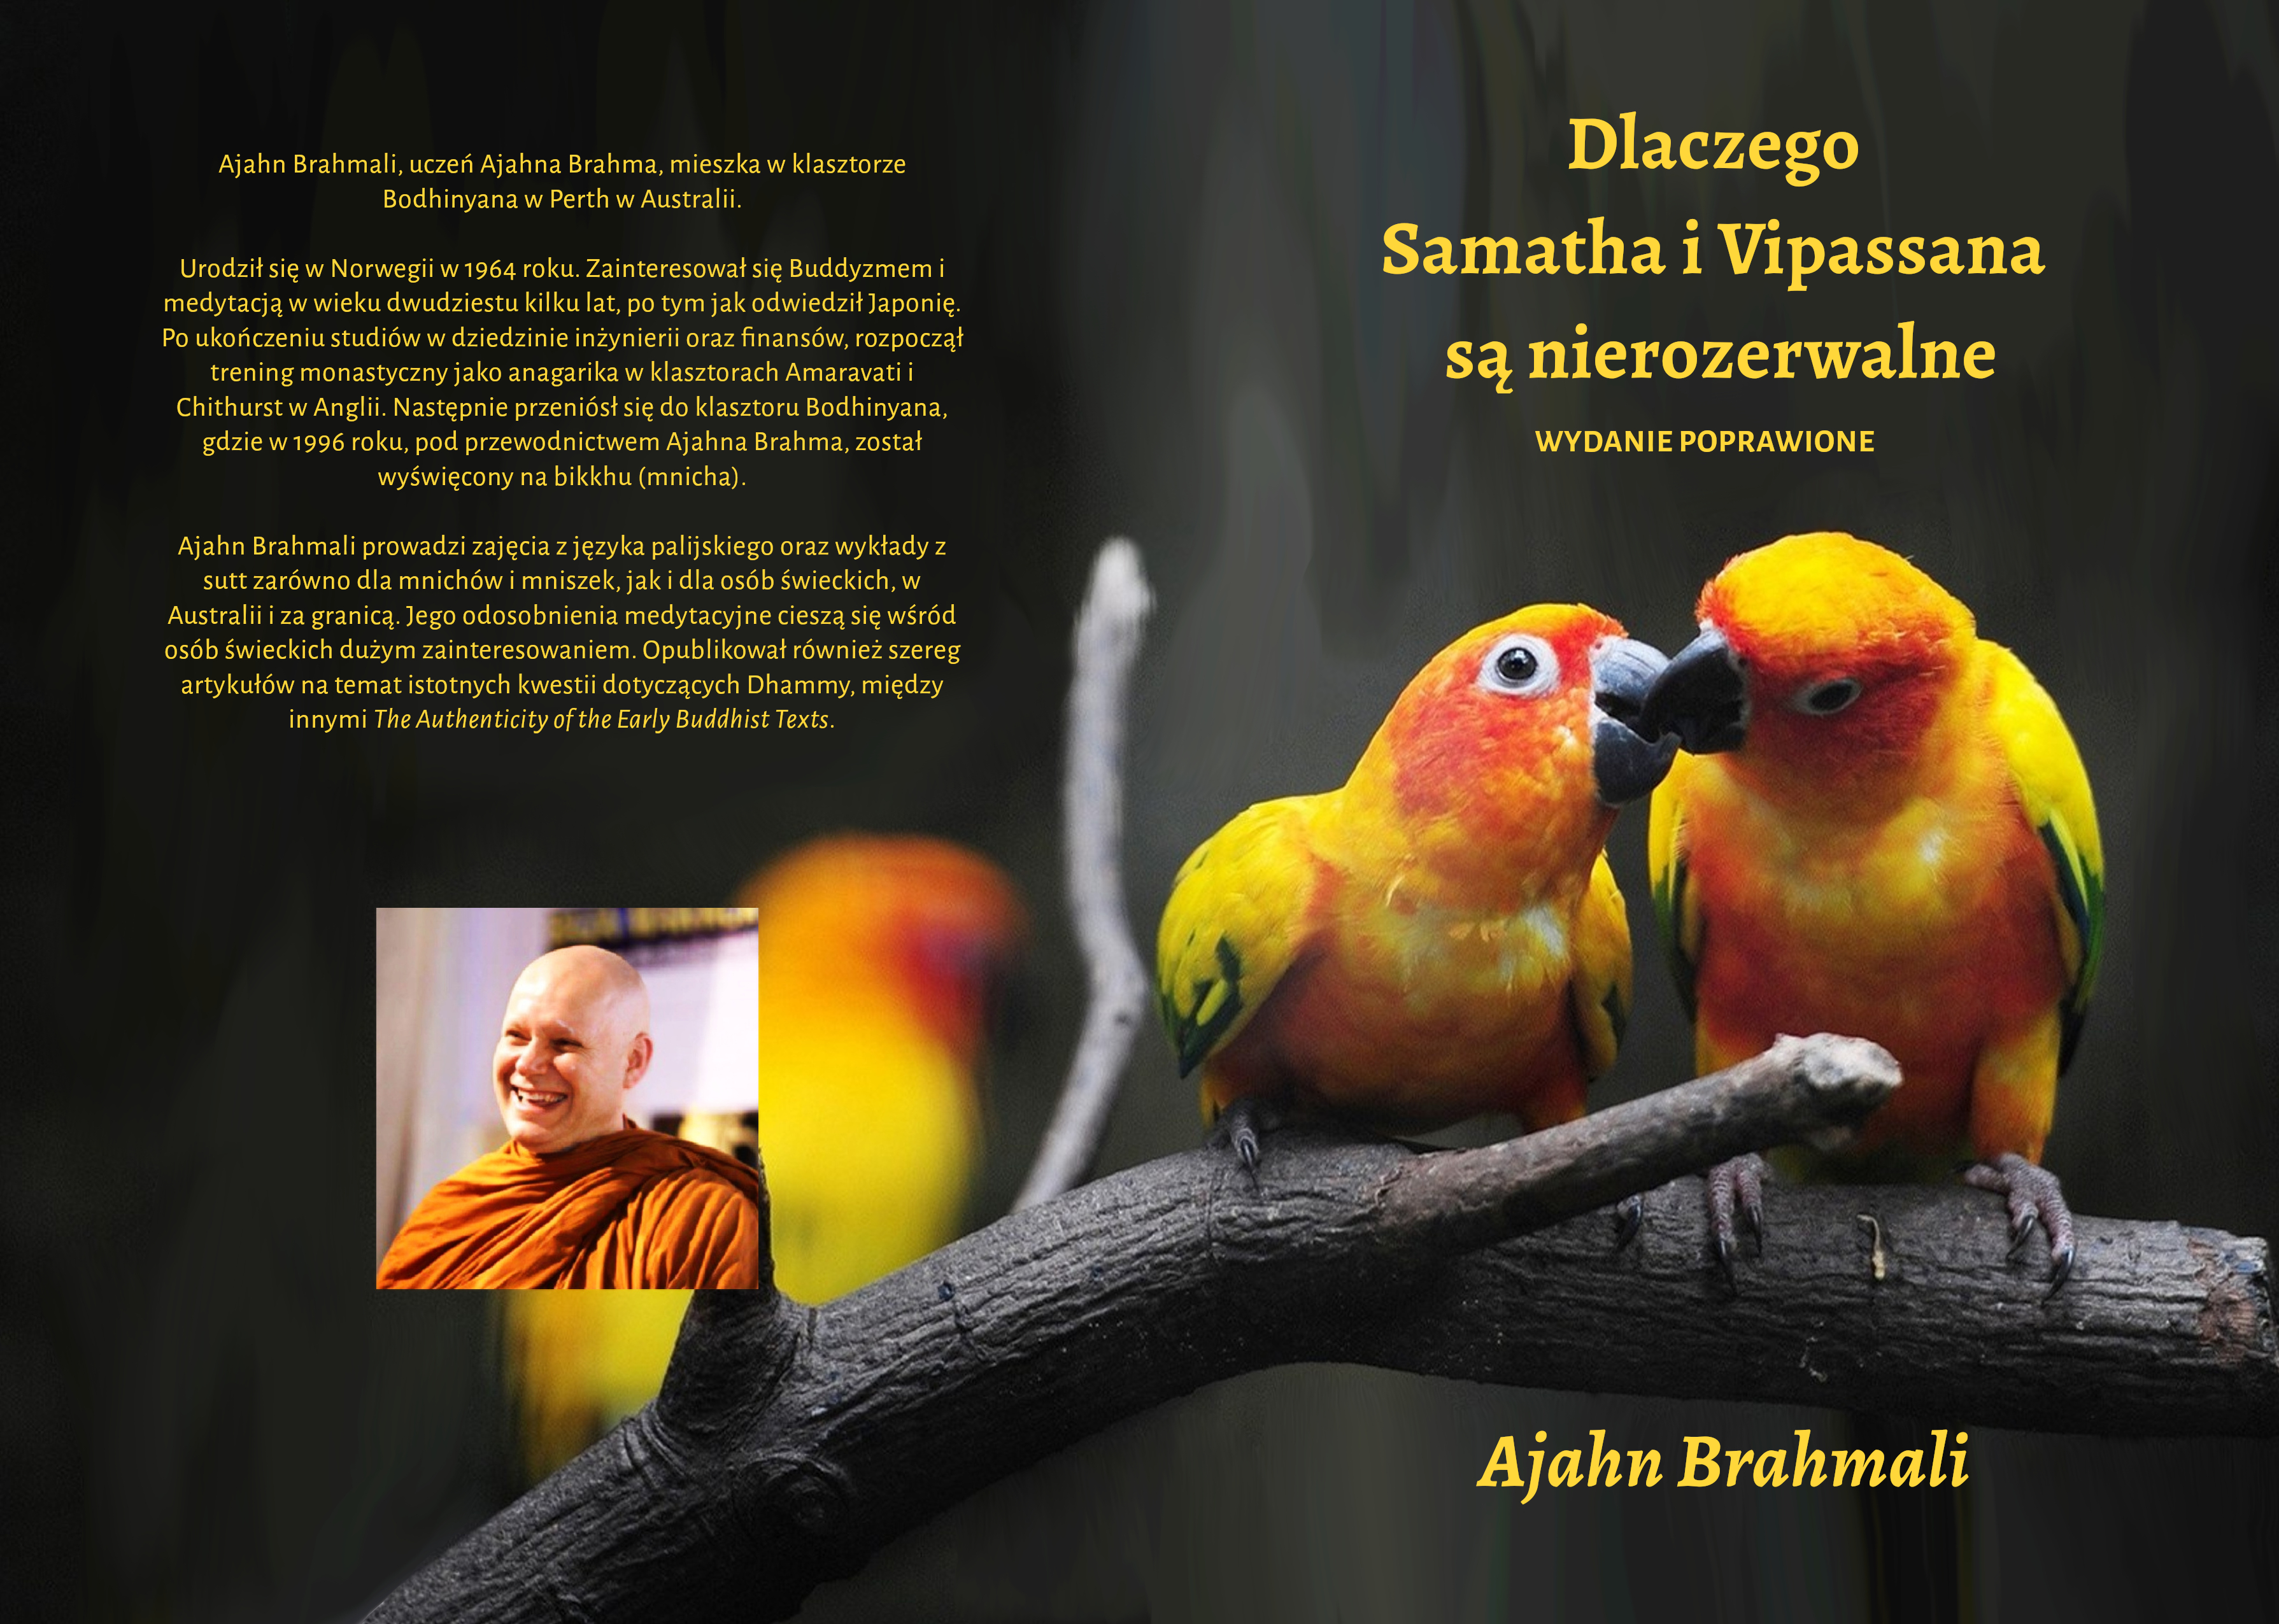
\includegraphics{sv-2_a5_cover.png}

\end{document}


